\section{Motivating Examples}\label{examples}

In this section we describe two motivating examples from the high-performance embedded system design domain. 
Modern heterogeneous embedded hardware platforms are notoriously difficult to design and to program. 
In this context, tool-supported model based approaches (e.g., Simulink, Ptolemy) are now widely acknowledged as some of the most 
effective approaches to designing embedded systems. 

Typically, these model-based approaches use tool chains that manipulate many different types of models. 
For example, structural platform description models range from system level models that abstract over processing and storage resource with their interconnections, to very low level Register-to-Logic level circuit models that are used to describe the structure of hardware accelerators within the platforms.

Similarly, behavioral description models range from application level modeling of the 
application using Models of Computation such as Synchronous Data Flow Graphs or 
Kahn Process Networks, to fine grain scalar operation level representations such as the 
basic-block level instruction dependence graph used in an optimizing compiler back-end. 

Most of these tool chains share a common goal: They aim to produce highly optimized  
implementations. This requires the use of advanced algorithms that implement very complex model manipulations. 
It is also the case that these manipulations often have similar algorithmic patterns. These patterns can be used as the basis for
developing reusable model transformations.


\subsection{Example 1: Using Model Types to Support Structural Substitutability}\label{structuralexample}

In the optimizing compiler domain, a variety of models describing different aspects of languages are manipulated (i.e., analyzed and transformed) at different stages of the compilation process. While the analyses and transformations are different, they also share many common characteristics.
For example, consider algorithms for schedule optimization. 
Obtaining an optimized implementation of an application on a target platform 
involves performing several static scheduling optimizations. 
Many of these algorithms have common characteristics, for example, they are often expressed as an acyclic graph resource constrained scheduling problem, for which many 
techniques (heuristics or MILP-Mixed Integer Linear Programming-solver based) have been proposed. 
Because these scheduling algorithms involve very sophisticated algorithms, reusable algorithms that can be tailored to the different types of representations (models) are highly desirable. 
For example, it would be useful to have a reusable scheduling algorithm that can be used to derive a schedule for an Application level Synchronous Data-flow graph on a multi-processor 
based implementation, as well as for generating efficient code for a customized VLIW (Very Long Instruction Word) embedded 
processor.        

However in this case, structural substitutability based only on constraints that can be expressed directly in a metamodel (e.g.,  multiplicity or element containment constraint) is not sufficient; other structural constraints need to be specified. 
For example, a classical static scheduling toolset can only operate on acyclic dependence graphs and the 
acyclicity property cannot be expressed directly in a metamodel. 
A language such as the Object Constraint Language (OCL) is needed to specify properties of acyclic graphs. 
In this case, model substitutability requires that a substitute model enforces the acyclicity constraint expressed in OCL.      
Model typing based on metamodels with OCL constraints can be used to enable such structural substitutability.

\subsection{Example 2: Using Model Types to Support Contract-based Behavioral Substitutability}\label{behavioralexample}

\subsubsection*{Behavioral substitutability for model transformations:}

A consistent scheduling tran-sformation must ensure that every node in the dependence graph is scheduled 
\emph{at least} once. This property can be expressed as a post-condition on the scheduling transformation and thus any scheduler 
implementation should enforce this post-condition. The effective post-condition could even be 
stricter; in our case we could consider a post-condition that restricts a node to be scheduled 
\emph{exactly} once.

% TODO steven : Figure for scheduling+mapping plus codegeb. 

The same holds for the pre-condition. For example, most schedulers operate on acyclic graphs and this can 
be translated as a pre-condition for the transformation. However, there also exists a class of 
pipelined schedulers that operate on cyclic graphs, in which cycles implement delays to preserve 
causality. For such pipelined schedulers, the pre-condition would not forbid cycles in the dependence graph.
That would, however, prevent a pipelined scheduler from being used to schedule 
acyclic graphs in a design flow.    

\subsubsection*{Contract based tool chain validation:}

An optimizing compiler custom tool chain consists of a sequence of analyses and transformations (called 
compiler passes) executed in a very carefully chosen order. They can hence be seen as a model 
transformation chain. Compiler passes cannot be combined arbitrarily, as each pass 
usually assumes that the program representation at hand has very specific properties.    

\begin{figure}[!t]
\centering
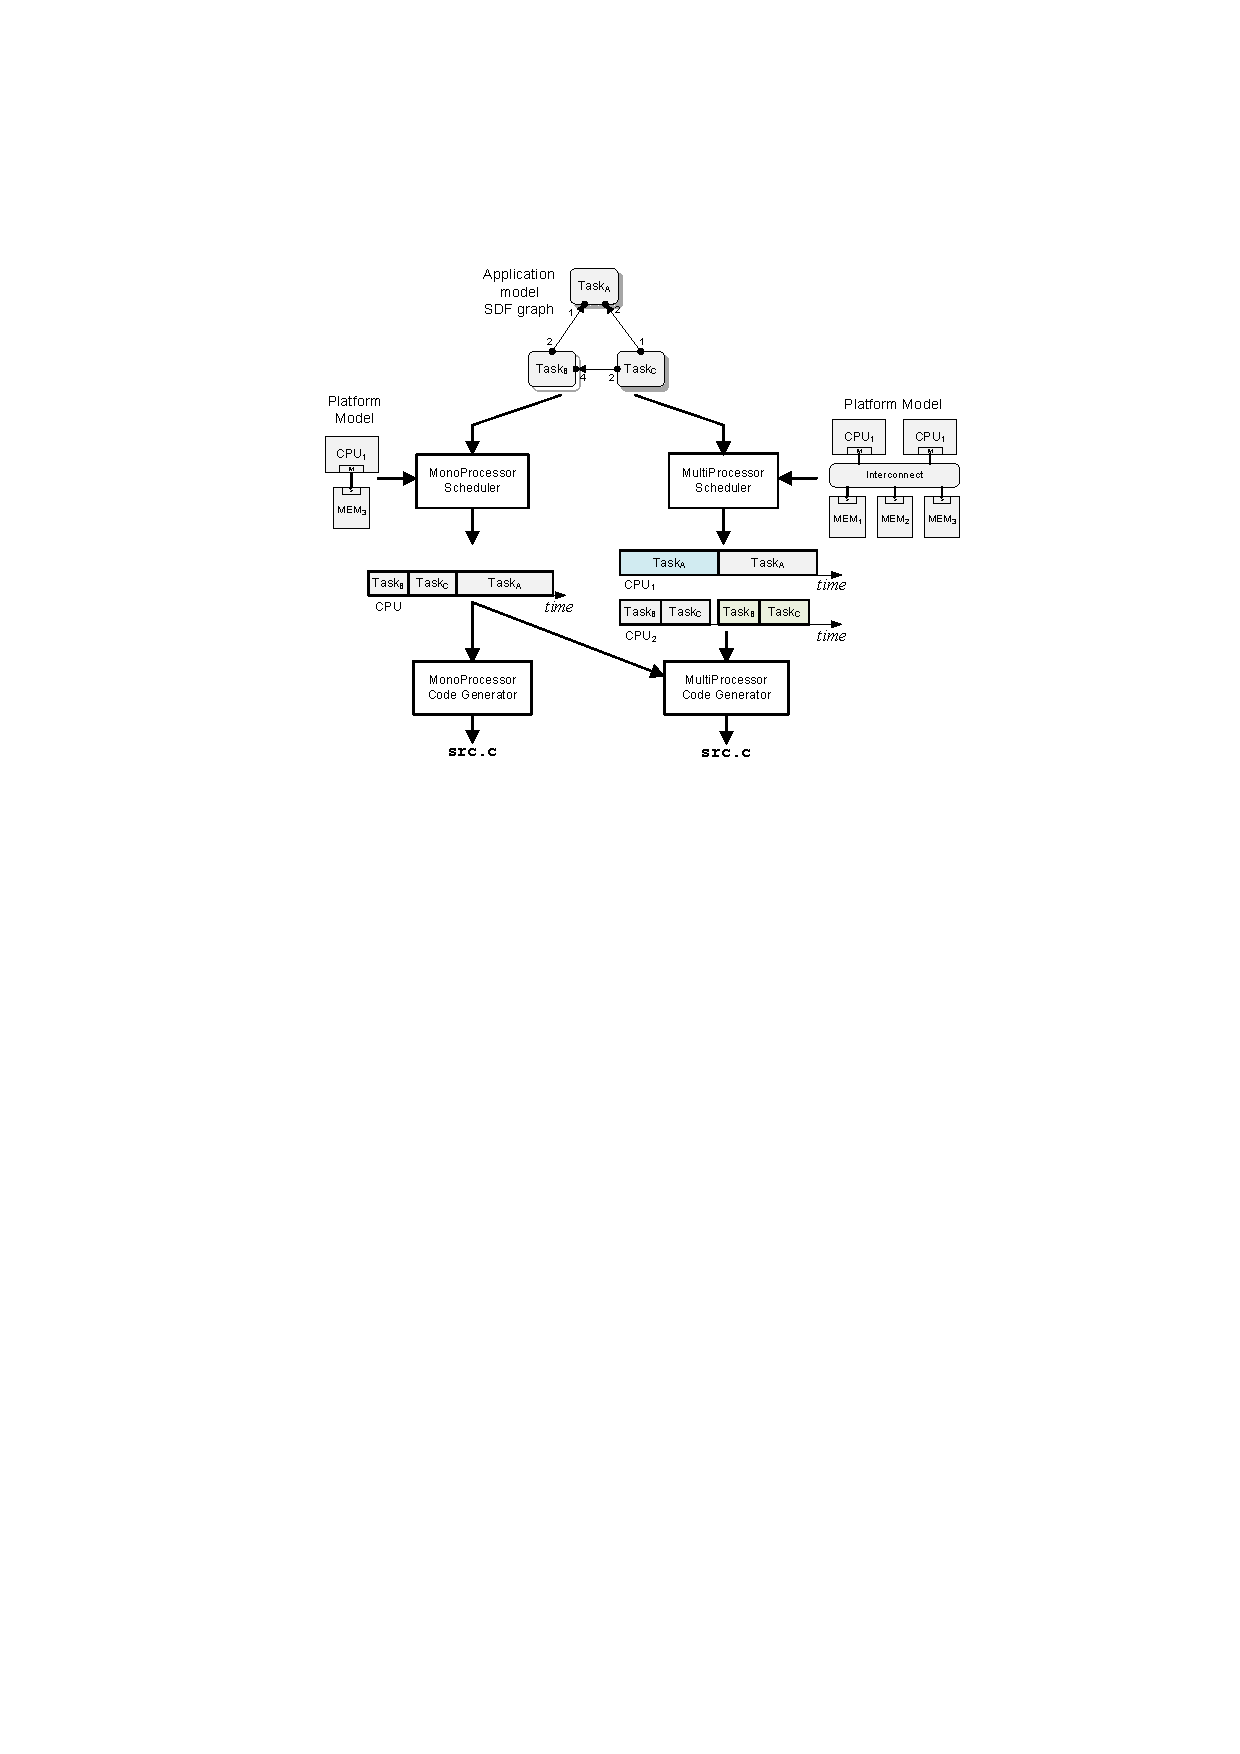
\includegraphics[width=4in]{fig/SDF-flow.pdf}
\caption{A Model based compiler tool chain for embedded multiprocessors. 
%The toolchain is used to   
%schedule a synchronous dataflow task graph on either a single or multi-processor depending 
%on the chosen scheduling component and platform model. Two back-end code generators are 
%provided. The monoprocessor code generator can only be used after a uniprocessor 
%scheduling stage, whereas the second back-end is more general and can be used for 
%both type of scheduling.     
}
\label{fig:toolchain}
\end{figure}


For example, consider a compiler tool chain for generating software code from 
Synchronous Data Flow Graph (SDF) model specifications on an embedded
platform. Such a tool chain is illustrated in Figure~\ref{fig:toolchain}.
Before any code can be produced, the SDF first needs to be scheduled on
this platform. Depending on whether the target system consists of a single or
several processors, it is likely that different scheduling algorithms will be
used. Similarly, different code generators (i.e. pretty printers) will have to
be used depending on whether we target a mono-processor or multiprocessor. Two back-end code generators are 
shown in Figure~\ref{fig:toolchain}. The mono-processor code generator can only be used after a mono-processor 
scheduling stage, whereas the second back-end is more general and can be used for 
both types of scheduling.     

These constraints -- that is targeting one or several processing resources --
apply to the result of the scheduling stage and to the input on the code
generation stage. They can hence be modeled as pre-conditions (resp.
post-conditions) expressed using OCL. When chaining a given scheduling and
code generation pass, we can ensure the consistency of the flow by checking if
the pre-/post-conditions of two chained transformation are satisfiable.



  